
\section*{Problema P7.28}

\renewcommand*\thesection{7.28}
\numberwithin{equation}{section}

\begin{center}
    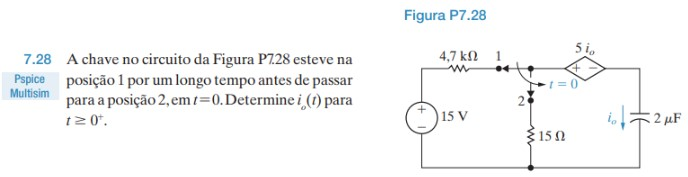
\includegraphics[scale=1.0]{P7.28.jpg}
\end{center}

Sabemos que a tensão em um capacitor é dada por	

\begin{equation}\label{eq:7.28.1}
    v(t) = C\diff{i}{t}
\end{equation}

****** PROBLEMA P 7.28 NAO ESTA NA LISTA !! *******

O CIRCUITO ESTA ABERTO EM T < 0, CAPACITOR FICA COMO CIRCUITO ABERTO EM CC
O primeiro passo é identificar a corrente $i_0(t)$ no estado inicial. Assim, aplicando análise de malhas com a chave na posição 1, usando $i_0$ como a corrente de malha,

\[ -15 + 4700i_0 + 5i_0 + C\diff{i_0}{t} = 0 \]

\[ \diff{i_0}{t} + \frac{4705}{C}i_0 = \frac{15}{C}\]

A EDO possui fator integrante $M(t)$ dado por 

\[ M(t) = e^{\int \frac{4705}{C} \, dt}  = e^{\frac{4705}{C}t} \]

Multiplicando ambos lados da EDO por $M(t)$, temos

\[ e^{\frac{4705}{C}t}\diff{i_0}{t} + e^{\frac{4705}{C}t}\frac{4705}{C}i_0 = e^{\frac{4705}{C}t} \frac{15}{C}\]

\[ \diff{\left[e^{\frac{4705}{C}t} \cdot i_0\right]}{t} = e^{\frac{4705}{C}t} \frac{15}{C}\]

\[ e^{\frac{4705}{C}t} \cdot i_0 = \int e^{\frac{4705}{C}t} \frac{15}{C} \, dt \]

\[ e^{\frac{4705}{C}t} \cdot i_0 = \frac{15}{C} \frac{C}{4705} \left(e^{\frac{4705}{C}t} + K\right) \]

\[ i_0(t) = e^{-\frac{4705}{C}t} \frac{15}{4705}\left(e^{\frac{4705}{C}t} + K\right) \]

\[ i_0(t) = 3.19 + 3.19Ke^{-\frac{4705}{C}t} \un{mA} \]










